\documentclass[../main.tex]{subfiles}
\begin{document}
\tikzstyle{container} = [draw, rectangle, inner sep=0.3cm, dashed, minimum height=3.5cm]
In the last 50 years car have transitioned from being composed only by mechanical parts to being completely stacked with electronics. The complexity of vehicles arises every year and the industry continuously raise the bar on the state of the art. The transitions to electro-mobility, the ADAS systems have done all but slowing down the development. The more a topic is market relevant, the higher the competition between companies, the faster the development in that field is going to be. The automakers are always ready to exploit or create new needs in order to adapt and attract customers. Automotive pulse of innovation and the "German Silicon Valley" is the place a engineer want to be to fell part of this complex, but for sure perfectly oiled machine.   
\begin{figure}
\centering
\begin{minipage}{.5\textwidth}
  \centering
  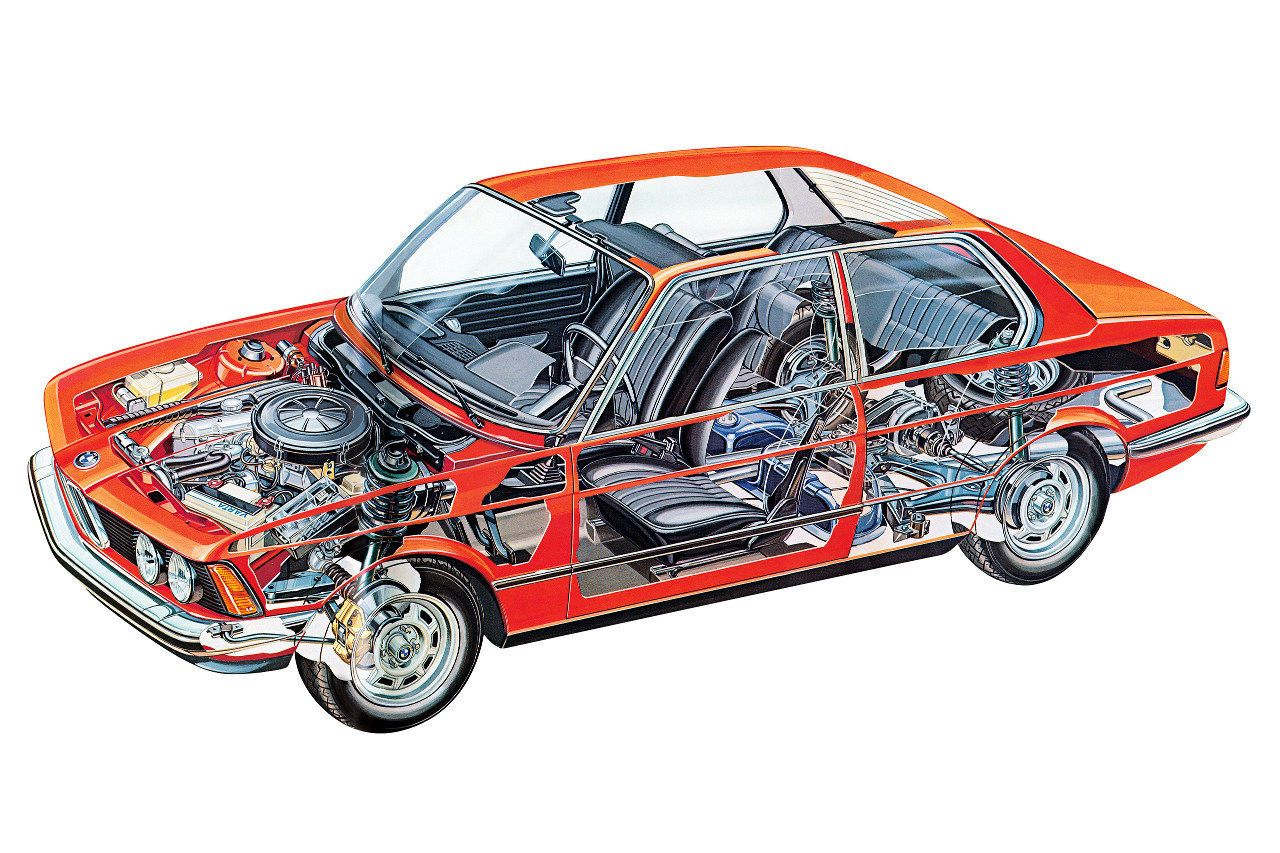
\includegraphics[width=6.3cm, height=4.8cm]{images_folder/4a56e1d50b56da42a10e29d451cf2b93.jpg}
  \caption{BMW 320 Coupe - 1975}
  \label{fig:test1}
\end{minipage}%
\begin{minipage}{.5\textwidth}
  \centering
  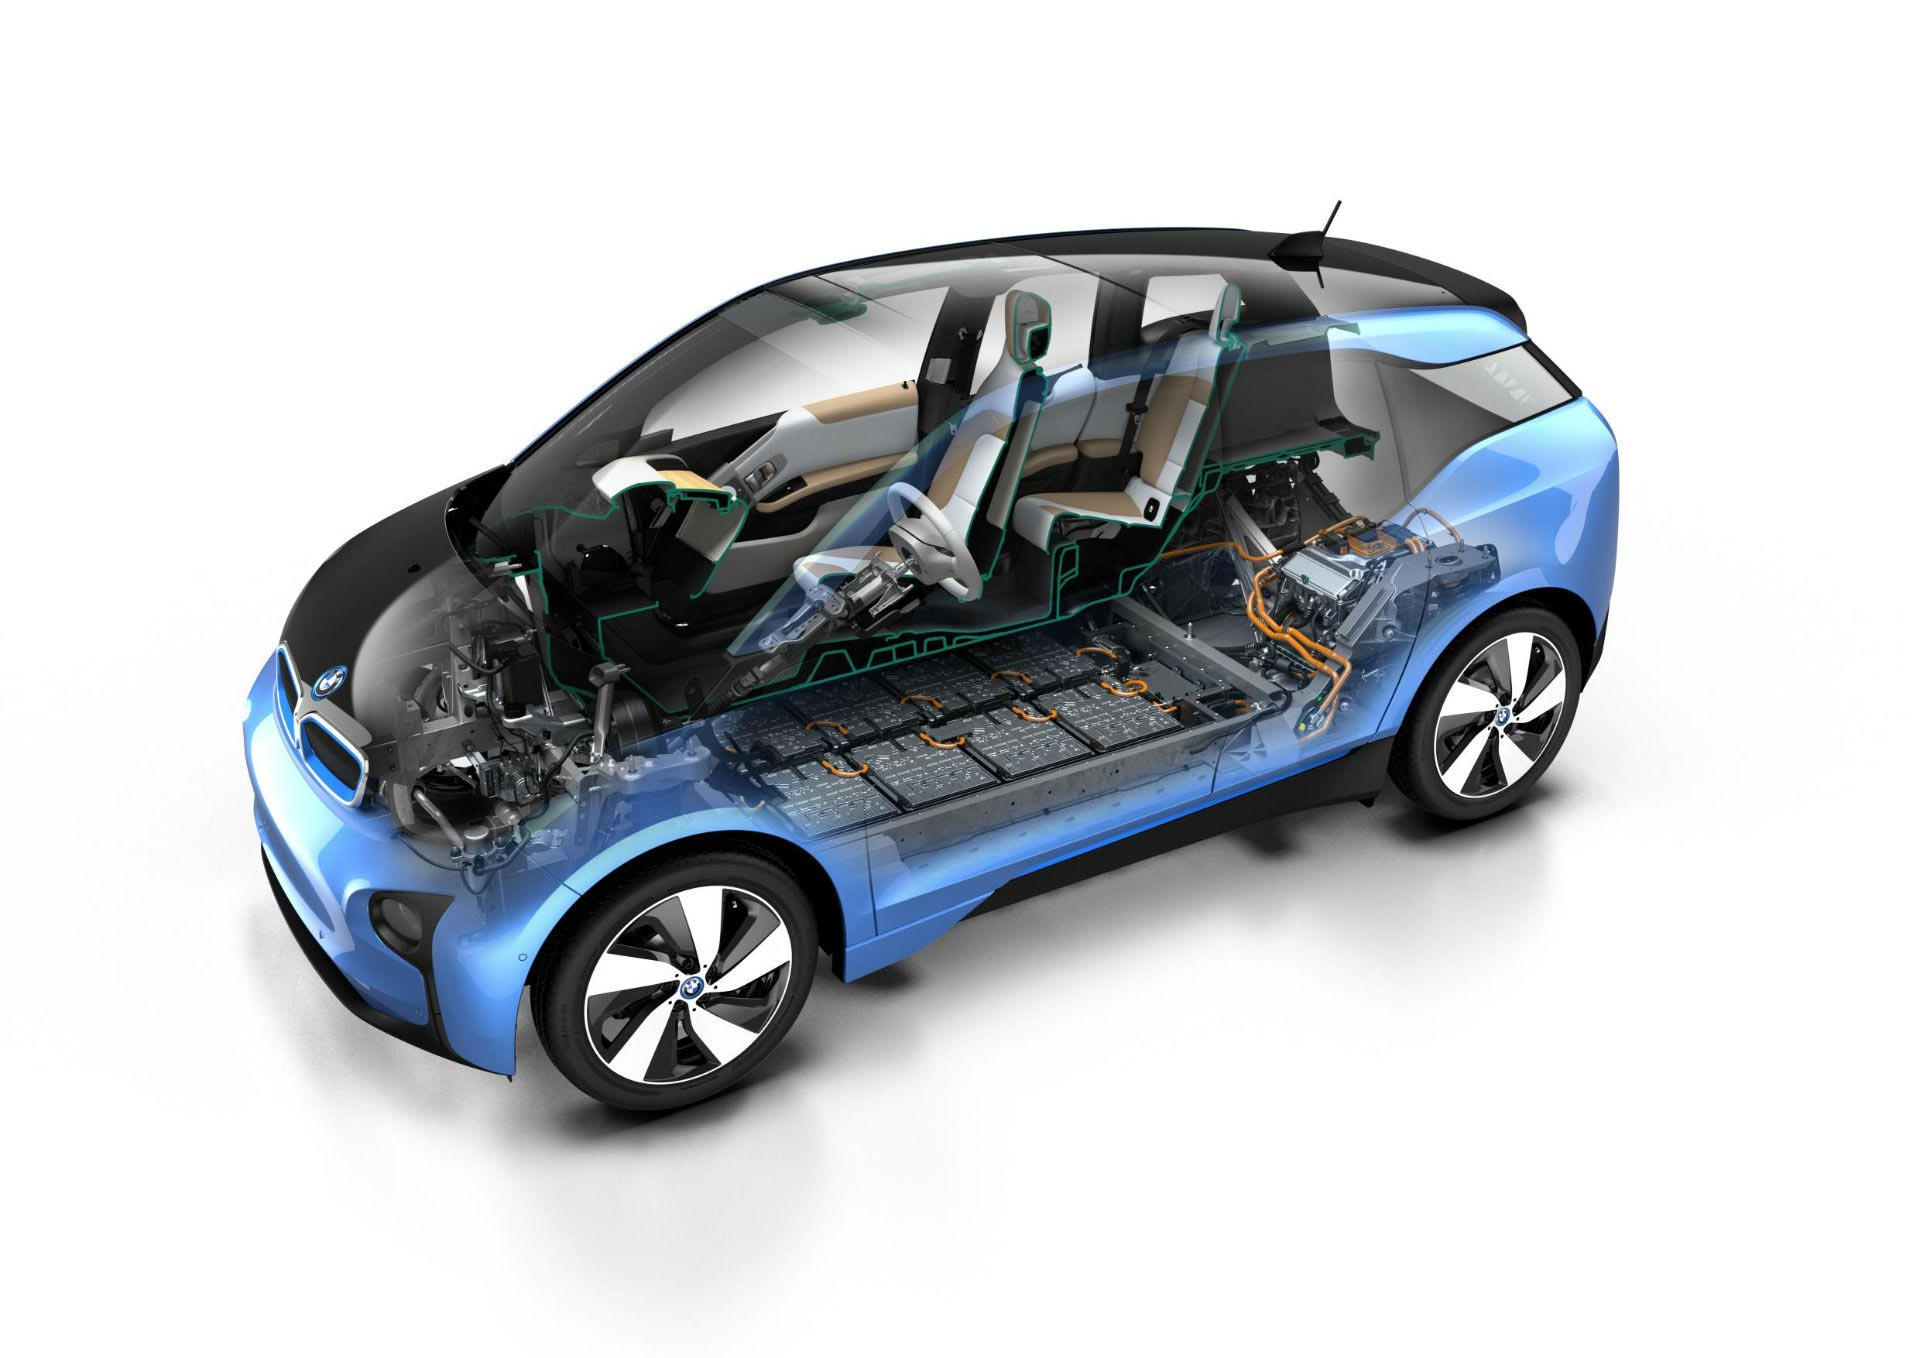
\includegraphics[width=6.3cm, height=4.8cm]{images_folder/BMW_i3.jpg}
  \caption{BMW I3 - 2015}
  \label{fig:test2}
\end{minipage}
\end{figure}

\section{Block Schema of a car}
The complexity of a \textit{vehicle system} can be easily simplified by block schemes. Block schemes are going to be a recursive topic during the thesis, thanks to the outside view that they allow to have over complexity.\\
    \begin{figure}[ht]
        \begin{center}
  \begin{tikzpicture}[auto, node distance=3cm,>=latex', scale=0.7,transform shape]
            \node [input1, name=input] {};
            \node [sum1, right=of input] (sum) {};
            \node [block1, right=of sum] (controller) {$Vehicle \;System$};
            \node [output, right=of controller] (output) {};
            \draw [draw,->] (input) -- node {$User\; inputs$} (sum);
            \draw [->] (sum) -- node {} (controller);
            \draw [->] (controller) -- node [name=y] {$(speed,\; position..)$}(output);
            \draw [->] (y) -- ++ (0,-3) -| node [pos=0.99] {$-$} (sum);
            \end{tikzpicture}
        \end{center}
    \caption{Block Scheme of a car}
    \end{figure}
    
The input to the \textit{vehicle system} can be an array of driver commands, such as the steering, throttle position and all the settings that control the car. The output of the system is not only the movement of the car, but also driver specific feelings such as the drive comfort or just the temperature in the vehicle. By further inspecting the system two blocks can be identified, the one responsible for the electronics and the one responsible for the mechanics. 
     \begin{figure}[ht]
        \begin{center}
  \begin{tikzpicture}[auto, node distance=3cm,>=latex', scale=0.7,transform shape]
            \node [input1, name=input] {};
            \node [sum1, right=of input] (sum) {};
            \node [sum, right=of sum] (sum_A) {};
            \node [block, right=of sum_A] (controller) {$Electronics$};
            \node [block, right=of controller] (mechanics) {$Mechanics$};
            \node [output1, right=of mechanics] (output) {};
            \draw [draw,->] (input) -- node {$User\; inputs$} (sum);
            \draw [->] (sum) -- node {} (sum_A);
            \draw [->] (sum_A) -- node {} (controller);
            \draw [->] (controller) -- node {} (mechanics);
            \draw [->] (mechanics) -- node [name=y] {$(speed,\; position..)$}(output);
            \draw [->] (mechanics) -- ++ (0,-2) -| node [pos=0.99] {$-$} (sum_A);
            \draw [->] (y) -- ++ (0,-4) -| node [pos=0.99] {$-$} (sum);
            % \node [container,fit=(controller) (mechanics) (sum_A)] (container) {};
            \end{tikzpicture}
        \end{center}
        \caption{Sub block division}
    \end{figure}       
These two blocks are strictly interconnected. The electronics drive the mechanics which output is given back as a feedback to correct the response. The system vehicle can be thought as a complex version of an embedded system where electronics drive mechanics following a logic described in lines of code.
Every mechanical component in cars has probably some electronic hardware related to it which is controlled by one of the many ECUs (Electronic control Units) present in the vehicle. The logic behind the control is embedded in lines of code. The yearly increase in lines of code for cars reported in Fig.\ref{fig:yearlyincreas} is a statement to this growth. 
\begin{figure}[H]
    \centering
    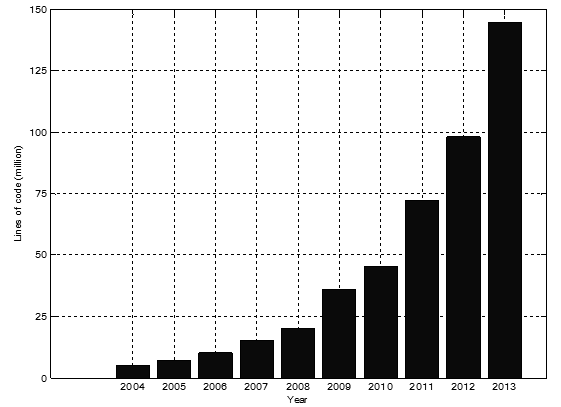
\includegraphics[width=0.6\linewidth]{images_folder/Yearly-increase-in-automotive-software-complexity-shown-by-million-lines-of-code-of-1-ConvertImage.png}
    \caption{Yearly increase in automotive software complexity}
    \label{fig:yearlyincreas}
\end{figure}
With more code comes an increasing complexity in the development process, which translate to challenges such as higher scalability and portability demands. The Thesis is going to focus on how this software is developed, generated and adapted to different ECUs by Automakers.
\section{ECU software}
The development of Software for ECUs is an extremely complex task, a single ECU can control up to a 1000 functions, and the number can be also higher for the control of complex parts, such as the motor.
Consider the following example. The function related to the control of the windshield wipers. In a scheme block manner we can see that the first indication comes from the driver, which activates the switch for the control of the windshield wipers. The signal travel to the ECU where it´s analyzed based on a logic stated in code lines. The output of the logic is then sent to the actuators specific board, which in this case actuates a motor that control the windshield wipers.\\
\begin{figure}[H]
    \centering
    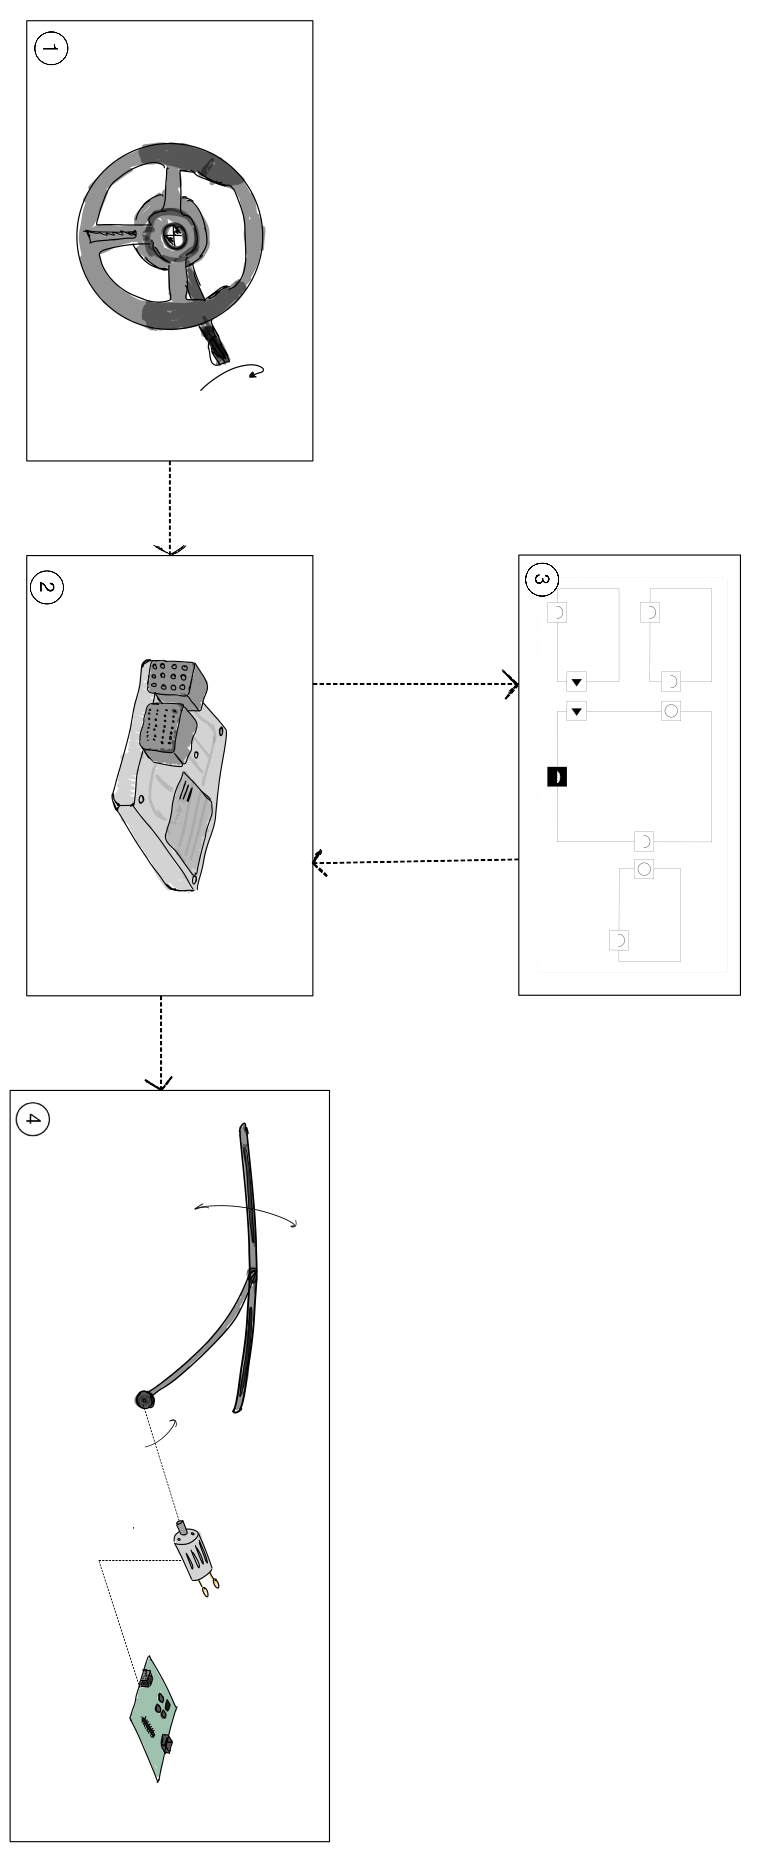
\includegraphics[width=0.45\linewidth, angle = 90]{images_folder/windshieldwipersfunction.jpeg}
    \caption{Windshield wipers function}
    \label{fig:WWFunct}
\end{figure}
The task seems like a basic one, consider now thousand of task sending contemporaneously information to the ECU. The ECU need to effectively elaborate thousand of input signals every second and output control information at a similar rate. In order to make everything work there are major problems that need to be considered:
\begin{itemize}
    \item Task prioritization, every function need to get a priority assigned, in order to be executed from the ECU. Priority need to be logically assigned by the ECU to each task. For example windshield wiping need to have a lower priority than airbag deployment. 
    \item Task scheduling, task need to be scheduled to meet deadlines, since ECUs are Real Time System, one of the requirements is that the system not only provide an output but this output respects certain time constraints.
    \item Access to shared resources, multiple task may require the ECU to read the same sensor or to act on the same actuator, or more deeply access the same memory location. The ECU need to control the access to these resources in order to avoid error but also to avoid saturation of the resources, which can lead to restarts and failures.  
    \item Failure handling, the ECU need to have the capabilities to avoid failure and to continue operating in case of failing hardware/software.
    \item Task predictability, task need to be designed to be predictable in the way they work, this allow to extend the predictability to the ensemble of tasks, and therefor predict the behaviour of the entire ECU in working conditions. 
\end{itemize}
The work of developing not only the logic behind tasks, but also the logic that control how task need to work in the system is one of the complex parts in the ECU design. In the next section an overview on this process is given. 
\subsection{ECU software design for tasks}
The design of software for a single function, such as the one reported in Fig.\ref{fig:WWFunct} is done by following the method of model based design approach. This technique, that uses as main tool the Mathworks Simulink package, introduce a level of abstraction between the code line and the logic, allowing for better software scalbility and portability. By using the Matlab Simulink tool the developer create the logic for the single function using blocks that need to describe the whole tasks functionality. The Simulink models, therefor comprises the following macro information:
\begin{itemize}
    \item Logical information, defines what the function actually does. 
    \item Integration information, how the function integrate with each other, which functions are related to the one developed. 
    \item Resources handling, like shared memory or communication interfaces as  the CAN bus
    \item IO capabilities, if a function require the read of particular sensors in order to compute the logic. 
\end{itemize}
All of those information are packed in Simulink blocks. Each function has its own Simulink file. Obviously all those information need to be transformed in ECU readable format. The Simulink block need to be compiled and transformed in executable code. This process of compilation of the code, with all the sub tasks related to it such as integration or testing is done in a in a step called software build. 
At BMW this is done via a dedicated software, internally developed in Python. The software takes as input all the functions and gives as an output the artifacts ready to be flashed in the ECU. In the next section an overview of this process is given.
\subsection{Build Process}
\label{subsection:Build process}
The build software has the function of compiling, linking, integrating, testing and validating the different functions developed for a certain ECU. In more details the task performed are the following:
\begin{itemize}
    \item Compilation and linking, the build compile the single function, generating executable code. 
    \item Architectural check, the build, after having compiled the functions, integrates them. For example multiple function can require the other ones. There is the need to check if a certain input or output is available for the required function and therefore test if the different function can integrate together.
    \item Quality checks, every software unit need to be test on Misra rules and other coding standards for developing safety-critical systems.
    \item Unit Testing and static code analysis, that analyze the software before this is compiled and deployed in the ECU.
    \item Documentation, generate documentation for every software components. 
    \item Artifacts archiving, the output artifacts need to be published in a repository.
\end{itemize}
\begin{figure}[H]
    \centering
    \begin{tikzpicture}[mindmap, grow cyclic, every node/.style=concept, concept color=gray!10, text width=]
    \node{Build}
    	child { node {Compilation}}
    	child { node {Architectural Check}}
    	child { node {Quality Checks}}
    	child { node {Documentation}}
    	child { node {Unit Testing}}
    	child { node {Linking}}
    	child { node {Artifacts Archiving}};
\end{tikzpicture}
    \caption{Caption}
    \label{fig:my_label}
\end{figure}
The output of a build run is provided by BMW to the actual ECU makers, such as Bosch and Vitesco. They add to the compiled software their part, closely related to the hardware that they develop. The complete software is flashed on the ECU. After having passed all the HIL testing, the ECU is homologated and enters production, to be later mounted on actual vehicles.
\section{Statement of Problem}
During the build process not only executable code is generated. Each step of the process is accompanied by the generation of data that not only describe the output artifact but gives important information on the results of each steps. It´s important also to highlight the fact that each of the process steps is supervised by different people if not different departments. The high load of data is shared over different departments and different developer. This makes it hard for each developer to have a 360 degree view of every step of the process, and how every step is going in terms of quality of the work. Even if the Agile like practices makes cooperation strong in between the teams,  a central overview on the process is missing.\\
A centralized overview would allow the developers to surf through different information regarding the whole development process. A way to efficiently give a overview of the process is via the use of a dashboard, that not only would allow for a graphical visualization but also for a way to centralize the data. In order to be useful inside a fast phased project the dashboard need to have the following characteristics:
\begin{itemize}
    \item Usability, the dashboard need to be easy to use and interactive, in the term that need to provide a rapid way to look for data from different sources. 
    \item Accessibility, all the team need to have access to the visualization.
    \item Real time data, the dashboard need to be backed by always updating data. This allow to have a real time picture of the full ECU software build. This is required because as multiple developer make changes on different parts of the process, the dashboard need to be able to quickly give a feedback of these changes.
    \item Trace-ability, keep track of how the different software releases compare to each other is possible via the storing of timestamped data. 
\end{itemize}
\section{Thesis Motivation}
The motivation behind the Thesis is related to the fact that in fast evolving environment, with multiple people required to cooperate together the creation of an overview on the process is crucial for allowing a better and more accurate feedback. 
The Thesis analyze the whole development process, in order to allow the reader to grasp the complexity of the process in which the work was developed. Then the actual active development part comes in, with an explanation of the procedure and a description of the output artifacts, in this case a dashboard.\\
A dashboard not only allow for an organization of the data but also to better non verbal interaction. The single developer can track the team accomplishment and therefore proceed in a less blind way. With the use of a dashboard each developer add another feedback loop to its own process, increasing the chances of eliminating the error and therefor developing better software, which translates to better products. It´s part of the automation definition the concept of reducing error by avoiding repetitive task, which is ultimately the goal of the dashboard. 
\section{Thesis Goals}
The main goals of the Thesis are:
\begin{itemize}
    \item Analyze the software development process for complex embedded system such the car ECU. Giving the reader an overview that allow to span from high level down to single tasks required. 
    \item Analyze the processes and methodology to tackle problem complexity. The reader is presented with Agile techniques and with other way to handle complexity in the software development environment.
    \item Relying on the two previous goal the reader is taken through the development of the main Thesis goal, a pipeline in which the data can automatically flow from the different processes to a software dashboard in which a interactive visualization of the data is given. 
\end{itemize}
\cleardoublepage
\end{document}